\begin{tikzpicture}

\GraphInit[vstyle=Classic]

\Vertex[Lpos=-90, x=0, y=0, L=$v$]{v};
\Vertex[Lpos=-90, x=2, y=0, L=$p_{1}$]{p1};
\Vertex[Lpos=-90, x=4, y=0, L=$p_{2}$]{p2};

\Edge[style ={-},label={$a_{1}$},labelstyle={above}]({v})({p1})
\Edge[style ={draw=none},label={$(a_{2})$},labelstyle={below}]({v})({p1})
\Edge[style ={-},label={$a_{2}$},labelstyle={above}]({p1})({p2})
\Edge[style ={draw=none},label={$(a_{3})$},labelstyle={below}]({p1})({p2})

\end{tikzpicture}
